\subsection{Action Node: Katana \& Scout}

The action node in reality corresponds to two ROS nodes working in parallel, the katana\_controller and the scout\_controller, both subscribing to the \textbackslash commands topic published by the decision node and processing that information into low level orders to the robots.

Both these nodes after completing a command from the Decision node send a "Done" message indicating they are ready for a new command.

\subsubsection{Katana}

%As mentioned in section \ref{Material: Katana} with help of the \textit{ROS} package \textit{Katana Native Interface} it is possible to power-off the motors of the robotic arm while keeping the robot communicating with the computer.

The Katana drivers already allow us to just send a setting for each it's joints and it will calculate the movement it needs to make to reach the goal. 

Through an empirical approach we determine the positions needed to form a trajetory that would lead to human like movements for different gestures.

While the motors are off, one can move the arm to the desired positions and afterwards read the values of the joint positions. Doing this repeatedly using all the desired positions, it is possible to program movement sequences, creating a gesture. After having each step of the movement, we programmed the maximum time for executing each step of the gesture. As well as for the positions, these maximum times were empirically determined. In the end of each movement, Katana goes to a defined default position.

Using this line of thought we created the following gestures: 

\begin{itemize}
\item high-five;
\item low-five; 
\item clap;
\item pass slied;
\item wave;
\item grab;
\end{itemize}

Since Katana as 7 degrees of freedom (6 joints and the gripper), the structures sent to the Katana are an array with 8 entries (The gripper receives two equal commands). Each entry is the angle in radians of each joint.

\begin{center}
General structure:
$\left[ Joint1, Joint2, ... , Joint6, Gripper_l Gripper_r\right]$
\end{center}

Using as an example the gesture "wave", the maximum time in seconds for reaching each position and the position goal sequence are given by:

\begin{center}
Maximum time: \\
$\left[5, 1.3, 1.3, 1.3, 5\right]$
\end{center}

\begin{table}[!ht]
\centering
\begin{tabular}{lc}
Position 1: & {[}-1.85, 1.57, 0.175, -0.35, -1.57, 0.175, 0.175{]} \\
Position 2: & {[}-1.85, 1.57, 0.175,  0.35, -1.57, 0.175, 0.175{]}  \\
Position 3: & {[}-1.85, 1.57, 0.175, -0.35, -1.57, 0.175, 0.175{]} \\
Position 4: & {[}-1.85, 1.57, 0.175,  0.35, -1.57, 0.175, 0.175{]}  \\
Position 5: & Default Position                                    
\end{tabular}
\end{table}

Looking at the table~ we can observe that in this movement the only joint that changes its position is Joint 4, similar to the human gesture where the only joint that moves while waving is the elbow joint.

\subsubsection{Scout}
The Scout robot is a two wheel, two motor differential drive robot, that means that for controlling the robot, we can use as parameters the linear and the angular velocity. One can translate these to the velocities of each wheel by using following equations:
\begin{equation}
v_{lin} = \frac{(\omega_{right}+\omega_{left})r}{2} \\
\end{equation}
\begin{equation}
v_{ang} = \omega = \frac{(\omega_{right}-\omega_{left})r}{2d}
\end{equation}
Where $r$ represents the radius of the wheel, and $d$ the distance between wheels.
As it can be seen in figure \ref{fig:scout_axis} our robot has two degrees of freedom, but since the movement of the robot isn't the main point of this project, we assume movement only in the \textit{x}-axis (forwards and backwards).

The implemented controller receives as an input only the distance in \textit{x} to the goal. Ideally the input would be the final position of the robot in the world map, we leave this as a possible improvement as it would the robot to be tracked by the Kinect Node.

\begin{figure}[!ht]
    \centering
    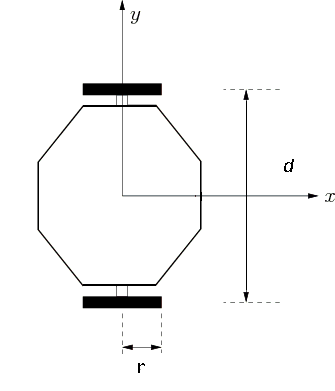
\includegraphics[width=0.5\columnwidth]{./ScoutAxis.png}
    \caption{Scout Axis}
    \label{fig:scout_axis}
\end{figure}

The control loop that we implemented looks as shown in figure \ref{fig:scout_loop}.

\begin{figure}[!ht]
    \centering
    \includegraphics[width=\columnwidth]{./ControlLoopScout.png}
    \caption{Scout's Control Loop}
    \label{fig:scout_loop}
\end{figure}
